\section{الگوریتم \lr{PPO}}
\label{sec:ppo_results}

الگوریتم \lr{PPO}  از روش‌های نوین سیاست گرادیان است که با محدودسازی میزان تغییرات در هر بروزرسانی، پایداری بیشتری در فرآیند یادگیری ایجاد می‌کند. در ادامه، عملکرد این الگوریتم در دو حالت مورد بررسی قرار گرفته است.

\subsection{مسیر طی‌شده}
\begin{figure}[H]
	\centering
	
	% سطر اول
	\subfloat[\lr{PPO} استاندارد]{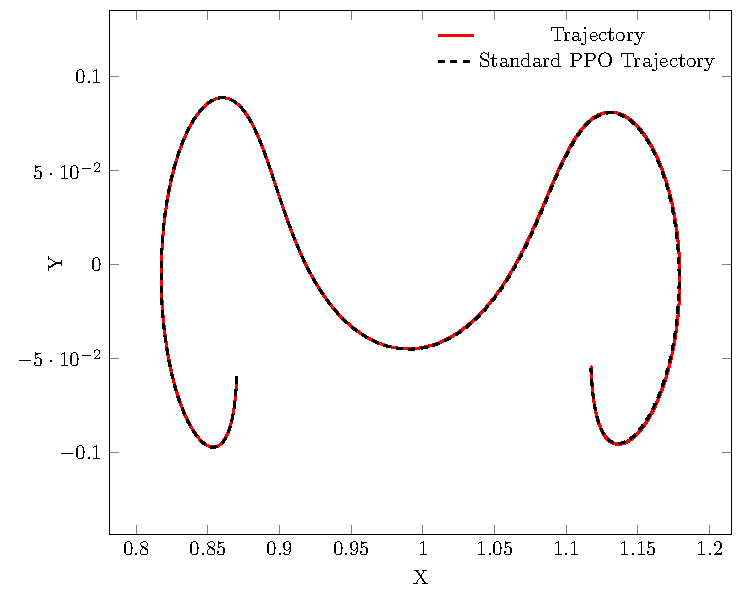
\includegraphics[width=.45\textwidth]{plots/ppo/trajectory_force/plot_trajectory.pdf}}%
	\subfloat[\lr{MA-PPO} بازی مجموع‌صفر]{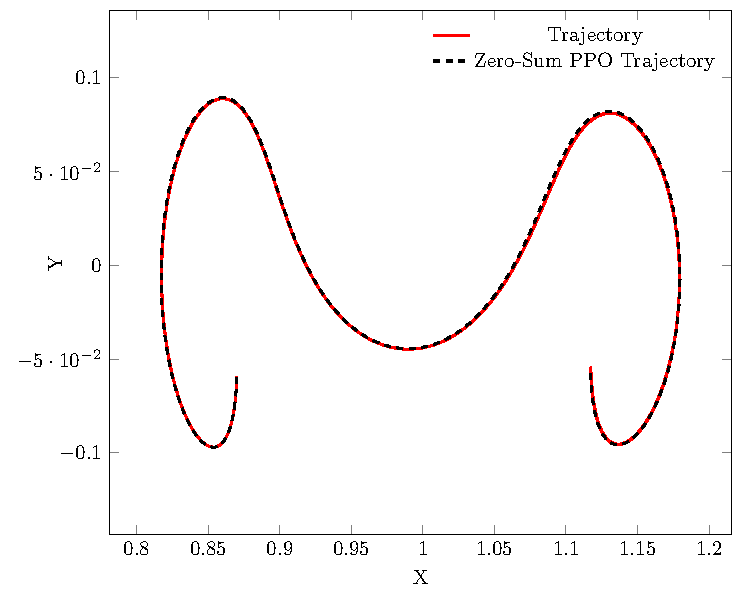
\includegraphics[width=.45\textwidth]{plots/ppo/trajectory_force/plot_trajectory_zs.pdf}}%
	
	\caption{مسیر طی‌شده فضاپیما با \lr{PPO} استاندارد و نسخه بازی مجموع‌صفر \lr{MA-PPO}.}
\end{figure}

\subsection{مسیر و فرمان پیشران}
\begin{figure}[H]
	\centering
	
	% سطر اول
	\subfloat[\lr{PPO} استاندارد]{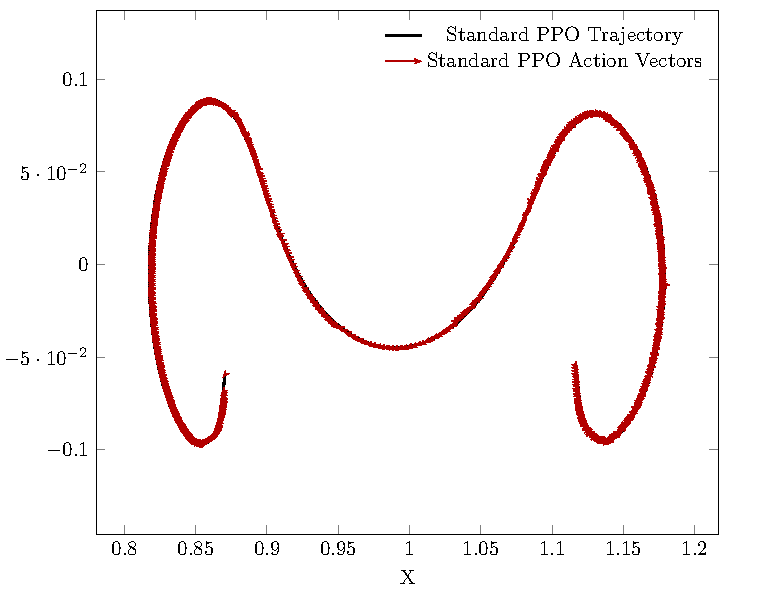
\includegraphics[width=.45\textwidth]{plots/ppo/trajectory_force/plot_trajectory_force.pdf}}%
	\subfloat[\lr{MA-PPO} بازی مجموع‌صفر]{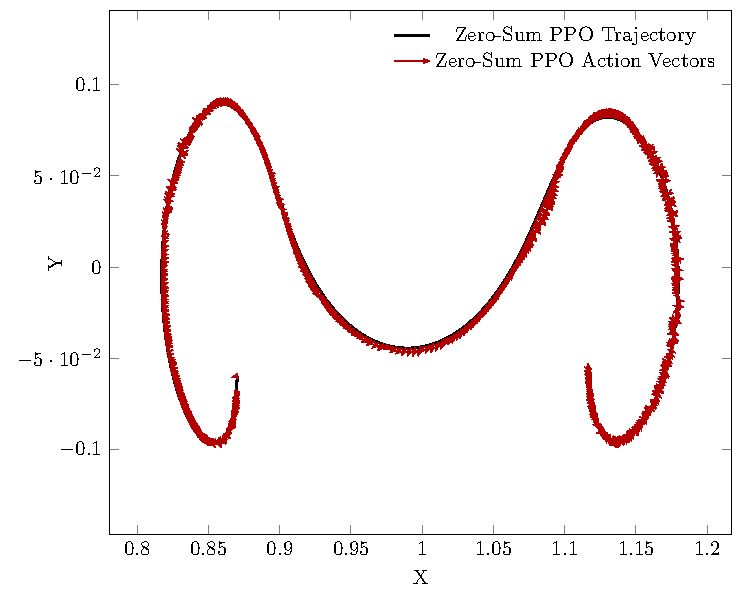
\includegraphics[width=.45\textwidth]{plots/ppo/trajectory_force/plot_trajectory_force_zs.pdf}}%
	
	\caption{مسیر و فرمان پیشران فضاپیما در \lr{PPO} استاندارد و نسخه بازی مجموع‌صفر \lr{MA-PPO}.}
\end{figure}

\subsection{توزیع پاداش تجمعی}
\begin{figure}[H]
	\centering
	
	% سطر اول
	\subfloat[شرایط اولیه تصادفی]{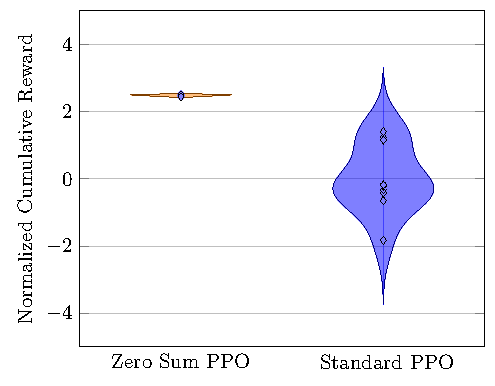
\includegraphics[width=.33\textwidth]{plots/ppo/violin_plot/initial_condition_shift.pdf}}%
	\subfloat[اغتشاش در عملگرها]{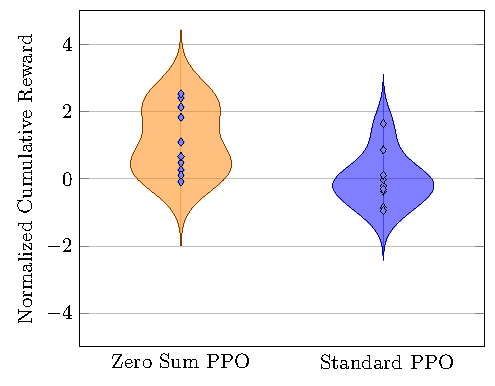
\includegraphics[width=.33\textwidth]{plots/ppo/violin_plot/actuator_disturbance.pdf}}%
	\subfloat[عدم تطابق مدل]{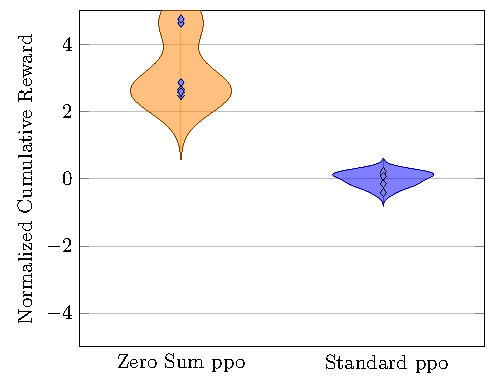
\includegraphics[width=.33\textwidth]{plots/ppo/violin_plot/model_mismatch.pdf}}\\[1ex]
	
	% سطر دوم
	\subfloat[مشاهده ناقص]{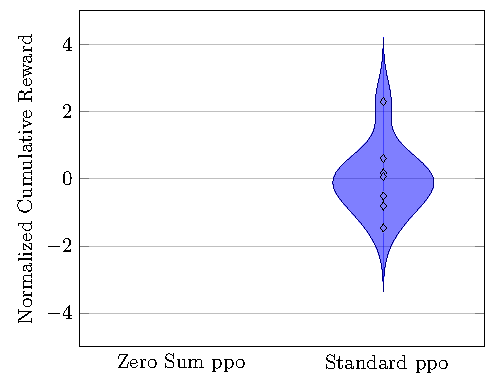
\includegraphics[width=.33\textwidth]{plots/ppo/violin_plot/partial_observation.pdf}}%
	\subfloat[نویز حسگر]{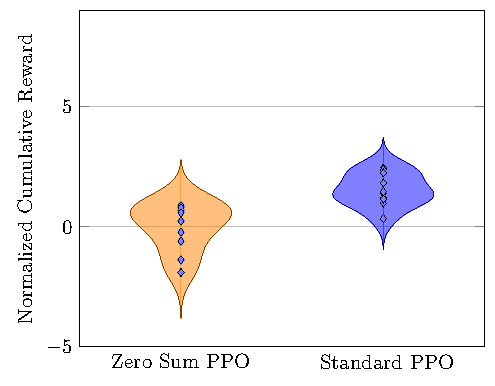
\includegraphics[width=.33\textwidth]{plots/ppo/violin_plot/sensor_noise.pdf}}%
	\subfloat[تأخیر زمانی]{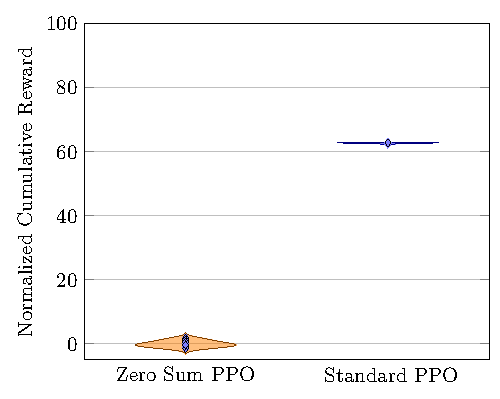
\includegraphics[width=.33\textwidth]{plots/ppo/violin_plot/time_delay.pdf}}
	
	\caption{مقایسه توزیع پاداش تجمعی برای \lr{PPO} و \lr{MA-PPO} در سناریوهای مختلف.}
	\label{fig:ppo_robustness_violin}
\end{figure}

\subsection{مقایسه عددی}
\begin{table}[H]
	\centering
	\setlength{\tabcolsep}{3pt}
	\small
	\begin{tabular}{@{} R{3.2cm} *{8}{C{1.05cm}} @{}}
		\toprule
		\multirow{2}{*}{\makecell[r]{سناریو}}
		& \multicolumn{2}{c}{پاداش تجمعی} & \multicolumn{2}{c}{مجموع خطای مسیر}
		& \multicolumn{2}{c}{مجموع تلاش کنترلی} & \multicolumn{2}{c}{احتمال شکست} \\
		\cmidrule(lr){2-3}\cmidrule(lr){4-5}\cmidrule(lr){6-7}\cmidrule(lr){8-9}
		& {\rotatebox[origin=c]{90}{\lr{PPO}}} & {\rotatebox[origin=c]{90}{\lr{MA-PPO}}}
		& {\rotatebox[origin=c]{90}{\lr{PPO}}} & {\rotatebox[origin=c]{90}{\lr{MA-PPO}}}
		& {\rotatebox[origin=c]{90}{\lr{PPO}}} & {\rotatebox[origin=c]{90}{\lr{MA-PPO}}}
		& {\rotatebox[origin=c]{90}{\lr{PPO}}} & {\rotatebox[origin=c]{90}{\lr{MA-PPO}}} \\
		\midrule
		شرایط اولیه تصادفی
		&
		$-1.85$ & ${0.46}$ & $0.22$ & ${0.14}$ & $1.98$ & $1.98$ & $0.70$ & ${0.00}$ \\
		اغتشاش در عملگرها
		&
		$-1.97$ & ${-1.91}$ & $8.33$ & ${7.50}$ & $3.42$ & $3.42$ & $1.00$ & $1.00$ \\
		عدم تطابق مدل
		&
		${0.46}$ & $0.30$ & ${0.07}$ & $0.08$ & $1.13$ & $1.13$ & $0.00$ & $0.00$ \\
		مشاهده ناقص
		&
		$-3.60$ & ${-1.81}$ & $2.34$ & ${2.06}$ & $2.15$ & $2.15$ & $1.00$ & $1.00$ \\
		نویز حسگر
		&
		${0.52}$ & $0.48$ & ${0.13}$ & $0.15$ & $2.08$ & $2.08$ & $0.00$ & $0.00$ \\
		تأخیر زمانی
		&
		${0.58}$ & $-2.44$ & ${0.03}$ & $2.49$ & $2.56$ & $2.56$ & ${0.00}$ & $1.00$ \\
		\bottomrule
	\end{tabular}
	\caption{مقایسه عملکرد \lr{PPO} و \lr{MA-PPO} در سناریوهای مختلف مقاومت}
	\label{tab:ppo_comparison}
\end{table}

نتایج نشان می‌دهد که الگوریتم \lr{PPO} در حالت بازی مجموع‌صفر عملکرد قابل توجهی دارد، اما تفاوت آن با نسخه استاندارد کمتر از \lr{DDPG} است. این می‌تواند به دلیل ماهیت ذاتی \lr{PPO} در ایجاد تعادل بین اکتشاف و بهره‌برداری باشد که آن را در حالت استاندارد نیز نسبتاً مقاوم می‌سازد.